% Options for packages loaded elsewhere
\PassOptionsToPackage{unicode}{hyperref}
\PassOptionsToPackage{hyphens}{url}
%
\documentclass[
  ignorenonframetext,
]{beamer}
\usepackage{pgfpages}
\setbeamertemplate{caption}[numbered]
\setbeamertemplate{caption label separator}{: }
\setbeamercolor{caption name}{fg=normal text.fg}
\beamertemplatenavigationsymbolsempty
% Prevent slide breaks in the middle of a paragraph
\widowpenalties 1 10000
\raggedbottom
\setbeamertemplate{part page}{
  \centering
  \begin{beamercolorbox}[sep=16pt,center]{part title}
    \usebeamerfont{part title}\insertpart\par
  \end{beamercolorbox}
}
\setbeamertemplate{section page}{
  \centering
  \begin{beamercolorbox}[sep=12pt,center]{part title}
    \usebeamerfont{section title}\insertsection\par
  \end{beamercolorbox}
}
\setbeamertemplate{subsection page}{
  \centering
  \begin{beamercolorbox}[sep=8pt,center]{part title}
    \usebeamerfont{subsection title}\insertsubsection\par
  \end{beamercolorbox}
}
\AtBeginPart{
  \frame{\partpage}
}
\AtBeginSection{
  \ifbibliography
  \else
    \frame{\sectionpage}
  \fi
}
\AtBeginSubsection{
  \frame{\subsectionpage}
}
\usepackage{lmodern}
\usepackage{amsmath}
\usepackage{ifxetex,ifluatex}
\ifnum 0\ifxetex 1\fi\ifluatex 1\fi=0 % if pdftex
  \usepackage[T1]{fontenc}
  \usepackage[utf8]{inputenc}
  \usepackage{textcomp} % provide euro and other symbols
  \usepackage{amssymb}
\else % if luatex or xetex
  \usepackage{unicode-math}
  \defaultfontfeatures{Scale=MatchLowercase}
  \defaultfontfeatures[\rmfamily]{Ligatures=TeX,Scale=1}
\fi
% Use upquote if available, for straight quotes in verbatim environments
\IfFileExists{upquote.sty}{\usepackage{upquote}}{}
\IfFileExists{microtype.sty}{% use microtype if available
  \usepackage[]{microtype}
  \UseMicrotypeSet[protrusion]{basicmath} % disable protrusion for tt fonts
}{}
\makeatletter
\@ifundefined{KOMAClassName}{% if non-KOMA class
  \IfFileExists{parskip.sty}{%
    \usepackage{parskip}
  }{% else
    \setlength{\parindent}{0pt}
    \setlength{\parskip}{6pt plus 2pt minus 1pt}}
}{% if KOMA class
  \KOMAoptions{parskip=half}}
\makeatother
\usepackage{xcolor}
\IfFileExists{xurl.sty}{\usepackage{xurl}}{} % add URL line breaks if available
\IfFileExists{bookmark.sty}{\usepackage{bookmark}}{\usepackage{hyperref}}
\hypersetup{
  pdftitle={tidyverse overview},
  pdfauthor={Andrew Ghazi},
  hidelinks,
  pdfcreator={LaTeX via pandoc}}
\urlstyle{same} % disable monospaced font for URLs
\newif\ifbibliography
\usepackage{color}
\usepackage{fancyvrb}
\newcommand{\VerbBar}{|}
\newcommand{\VERB}{\Verb[commandchars=\\\{\}]}
\DefineVerbatimEnvironment{Highlighting}{Verbatim}{commandchars=\\\{\}}
% Add ',fontsize=\small' for more characters per line
\usepackage{framed}
\definecolor{shadecolor}{RGB}{248,248,248}
\newenvironment{Shaded}{\begin{snugshade}}{\end{snugshade}}
\newcommand{\AlertTok}[1]{\textcolor[rgb]{0.94,0.16,0.16}{#1}}
\newcommand{\AnnotationTok}[1]{\textcolor[rgb]{0.56,0.35,0.01}{\textbf{\textit{#1}}}}
\newcommand{\AttributeTok}[1]{\textcolor[rgb]{0.77,0.63,0.00}{#1}}
\newcommand{\BaseNTok}[1]{\textcolor[rgb]{0.00,0.00,0.81}{#1}}
\newcommand{\BuiltInTok}[1]{#1}
\newcommand{\CharTok}[1]{\textcolor[rgb]{0.31,0.60,0.02}{#1}}
\newcommand{\CommentTok}[1]{\textcolor[rgb]{0.56,0.35,0.01}{\textit{#1}}}
\newcommand{\CommentVarTok}[1]{\textcolor[rgb]{0.56,0.35,0.01}{\textbf{\textit{#1}}}}
\newcommand{\ConstantTok}[1]{\textcolor[rgb]{0.00,0.00,0.00}{#1}}
\newcommand{\ControlFlowTok}[1]{\textcolor[rgb]{0.13,0.29,0.53}{\textbf{#1}}}
\newcommand{\DataTypeTok}[1]{\textcolor[rgb]{0.13,0.29,0.53}{#1}}
\newcommand{\DecValTok}[1]{\textcolor[rgb]{0.00,0.00,0.81}{#1}}
\newcommand{\DocumentationTok}[1]{\textcolor[rgb]{0.56,0.35,0.01}{\textbf{\textit{#1}}}}
\newcommand{\ErrorTok}[1]{\textcolor[rgb]{0.64,0.00,0.00}{\textbf{#1}}}
\newcommand{\ExtensionTok}[1]{#1}
\newcommand{\FloatTok}[1]{\textcolor[rgb]{0.00,0.00,0.81}{#1}}
\newcommand{\FunctionTok}[1]{\textcolor[rgb]{0.00,0.00,0.00}{#1}}
\newcommand{\ImportTok}[1]{#1}
\newcommand{\InformationTok}[1]{\textcolor[rgb]{0.56,0.35,0.01}{\textbf{\textit{#1}}}}
\newcommand{\KeywordTok}[1]{\textcolor[rgb]{0.13,0.29,0.53}{\textbf{#1}}}
\newcommand{\NormalTok}[1]{#1}
\newcommand{\OperatorTok}[1]{\textcolor[rgb]{0.81,0.36,0.00}{\textbf{#1}}}
\newcommand{\OtherTok}[1]{\textcolor[rgb]{0.56,0.35,0.01}{#1}}
\newcommand{\PreprocessorTok}[1]{\textcolor[rgb]{0.56,0.35,0.01}{\textit{#1}}}
\newcommand{\RegionMarkerTok}[1]{#1}
\newcommand{\SpecialCharTok}[1]{\textcolor[rgb]{0.00,0.00,0.00}{#1}}
\newcommand{\SpecialStringTok}[1]{\textcolor[rgb]{0.31,0.60,0.02}{#1}}
\newcommand{\StringTok}[1]{\textcolor[rgb]{0.31,0.60,0.02}{#1}}
\newcommand{\VariableTok}[1]{\textcolor[rgb]{0.00,0.00,0.00}{#1}}
\newcommand{\VerbatimStringTok}[1]{\textcolor[rgb]{0.31,0.60,0.02}{#1}}
\newcommand{\WarningTok}[1]{\textcolor[rgb]{0.56,0.35,0.01}{\textbf{\textit{#1}}}}
\usepackage{graphicx}
\makeatletter
\def\maxwidth{\ifdim\Gin@nat@width>\linewidth\linewidth\else\Gin@nat@width\fi}
\def\maxheight{\ifdim\Gin@nat@height>\textheight\textheight\else\Gin@nat@height\fi}
\makeatother
% Scale images if necessary, so that they will not overflow the page
% margins by default, and it is still possible to overwrite the defaults
% using explicit options in \includegraphics[width, height, ...]{}
\setkeys{Gin}{width=\maxwidth,height=\maxheight,keepaspectratio}
% Set default figure placement to htbp
\makeatletter
\def\fps@figure{htbp}
\makeatother
\setlength{\emergencystretch}{3em} % prevent overfull lines
\providecommand{\tightlist}{%
  \setlength{\itemsep}{0pt}\setlength{\parskip}{0pt}}
\setcounter{secnumdepth}{-\maxdimen} % remove section numbering
\ifluatex
  \usepackage{selnolig}  % disable illegal ligatures
\fi

\title{tidyverse overview}
\author{Andrew Ghazi}
\date{March 25th 2021}

\begin{document}
\frame{\titlepage}

\begin{frame}[fragile]{While people are joining the meeting}
\protect\hypertarget{while-people-are-joining-the-meeting}{}
\begin{enumerate}
\tightlist
\item
  Install stuff
\end{enumerate}

\begin{itemize}
\tightlist
\item
  \href{rstudio.com}{Rstudio} - \texttt{rstudio.com}
\item
  the tidyverse with this R command:
  \texttt{install.packages("tidyverse")}
\end{itemize}

\begin{enumerate}
\setcounter{enumi}{1}
\tightlist
\item
  Get the slides and/or code if you'd like to follow along:
\end{enumerate}

\begin{itemize}
\tightlist
\item
  \url{github.com/andrewGhazi/tidy_overview}
\end{itemize}
\end{frame}

\begin{frame}[fragile]{What is the tidyverse?}
\protect\hypertarget{what-is-the-tidyverse}{}
\begin{itemize}
\item
  A dialect of R
\item
  A suite of R packages with a shared design philosophy
\item
  Install it with this R command:
  \texttt{install.packages(\textquotesingle{}tidyverse\textquotesingle{})}
\end{itemize}


\includegraphics[width=0.95\linewidth,height=0.95\textheight]{images/tidyverse-logo}
\end{frame}

\begin{frame}{Why use the tidyverse?}
\protect\hypertarget{why-use-the-tidyverse}{}
\begin{itemize}
\tightlist
\item
  Shared design philosophy --\textgreater{} consistency
\item
  Design goal: Lower your cognitive burden
\item
  Easy to learn, write, and read
\item
  Other people use it
\end{itemize}
\end{frame}

\begin{frame}[fragile]{A note}
\protect\hypertarget{a-note}{}
Lecture notes show up like this.

\begin{Shaded}
\begin{Highlighting}[]
\FunctionTok{print}\NormalTok{(}\StringTok{\textquotesingle{}R code looks like this.\textquotesingle{}}\NormalTok{)}
\end{Highlighting}
\end{Shaded}

\begin{verbatim}
## [1] "R code looks like this."
\end{verbatim}

\begin{Shaded}
\begin{Highlighting}[]
\FunctionTok{print}\NormalTok{(}\StringTok{\textquotesingle{}Console output has two pound symbols in front.\textquotesingle{}}\NormalTok{)}
\end{Highlighting}
\end{Shaded}

\begin{verbatim}
## [1] "Console output has two pound symbols in front."
\end{verbatim}

\begin{Shaded}
\begin{Highlighting}[]
\NormalTok{x }\OtherTok{=} \DecValTok{5} 
\end{Highlighting}
\end{Shaded}

Assignment prints nothing.
\end{frame}

\begin{frame}[fragile]{Load the tidyverse}
\protect\hypertarget{load-the-tidyverse}{}
The startup message lists loaded packages and overwritten functions.

\begin{Shaded}
\begin{Highlighting}[]
\FunctionTok{library}\NormalTok{(tidyverse)}
\end{Highlighting}
\end{Shaded}

\begin{verbatim}
## -- Attaching packages --------------------------------------- tidyverse 1.3.0 --
\end{verbatim}

\begin{verbatim}
## v ggplot2 3.3.3     v purrr   0.3.4
## v tibble  3.0.5     v dplyr   1.0.3
## v tidyr   1.1.2     v stringr 1.4.0
## v readr   1.4.0     v forcats 0.5.0
\end{verbatim}

\begin{verbatim}
## -- Conflicts ------------------------------------------ tidyverse_conflicts() --
## x dplyr::filter() masks stats::filter()
## x dplyr::lag()    masks stats::lag()
\end{verbatim}
\end{frame}

\begin{frame}[fragile]{Help}
\protect\hypertarget{help}{}
To look at the documentation for any function, use \texttt{?} or
\texttt{help()}

How to read help:
\url{https://socviz.co/appendix.html\#a-little-more-about-r}
\end{frame}

\hypertarget{basic-concepts}{%
\section{Basic concepts}\label{basic-concepts}}

\begin{frame}[fragile]{Data frames}
\protect\hypertarget{data-frames}{}
\begin{itemize}
\tightlist
\item
  Used to store ordered collections of variables
\end{itemize}

\begin{Shaded}
\begin{Highlighting}[]
\NormalTok{diabetes}
\end{Highlighting}
\end{Shaded}

\begin{verbatim}
## # A tibble: 532 x 8
##    npreg   glu    bp  skin   bmi   ped   age diabetic
##    <dbl> <dbl> <dbl> <dbl> <dbl> <dbl> <dbl> <chr>   
##  1     5    86    68    28  30.2 0.364    24 No      
##  2     7   195    70    33  25.1 0.163    55 Yes     
##  3     5    77    82    41  35.8 0.156    35 No      
##  4     0   165    76    43  47.9 0.259    26 No      
##  5     0   107    60    25  26.4 0.133    23 No      
##  6     5    97    76    27  35.6 0.378    52 Yes     
##  7     3    83    58    31  34.3 0.336    25 No      
##  8     1   193    50    16  25.9 0.655    24 No      
##  9     3   142    80    15  32.4 0.2      63 No      
## 10     2   128    78    37  43.3 1.22     31 Yes     
## # ... with 522 more rows
\end{verbatim}
\end{frame}

\begin{frame}[fragile]{tidy data}
\protect\hypertarget{tidy-data}{}
\begin{itemize}
\tightlist
\item
  Columns are variables
\item
  Rows are observations
\end{itemize}

\begin{verbatim}
## # A tibble: 532 x 8
##    npreg   glu    bp  skin   bmi   ped   age diabetic
##    <dbl> <dbl> <dbl> <dbl> <dbl> <dbl> <dbl> <chr>   
##  1     5    86    68    28  30.2 0.364    24 No      
##  2     7   195    70    33  25.1 0.163    55 Yes     
##  3     5    77    82    41  35.8 0.156    35 No      
##  4     0   165    76    43  47.9 0.259    26 No      
##  5     0   107    60    25  26.4 0.133    23 No      
##  6     5    97    76    27  35.6 0.378    52 Yes     
##  7     3    83    58    31  34.3 0.336    25 No      
##  8     1   193    50    16  25.9 0.655    24 No      
##  9     3   142    80    15  32.4 0.2      63 No      
## 10     2   128    78    37  43.3 1.22     31 Yes     
## # ... with 522 more rows
\end{verbatim}
\end{frame}

\begin{frame}[fragile]{Pipes}
\protect\hypertarget{pipes}{}
\begin{itemize}
\item
  Pipes look like this: \texttt{\%\textgreater{}\%}
\item
  They take the input from the left side, and hand it to the right side:
\end{itemize}

\begin{Shaded}
\begin{Highlighting}[]
\FunctionTok{c}\NormalTok{(}\DecValTok{1}\NormalTok{,}\DecValTok{2}\NormalTok{,}\DecValTok{3}\NormalTok{,}\DecValTok{4}\NormalTok{) }\SpecialCharTok{\%\textgreater{}\%}\NormalTok{ mean}
\end{Highlighting}
\end{Shaded}

\begin{verbatim}
## [1] 2.5
\end{verbatim}

\begin{itemize}
\item
  Verbalize as: ``and then''.
\item
  ``Set up this vector and then take the mean''.
\end{itemize}
\end{frame}

\begin{frame}{Pipe example}
\protect\hypertarget{pipe-example}{}
Why are pipes useful?
\end{frame}

\begin{frame}{Pipe example}
\protect\hypertarget{pipe-example-1}{}
Why are pipes useful?


\includegraphics[width=0.75\linewidth]{images/top}
\end{frame}

\begin{frame}{Pipe example}
\protect\hypertarget{pipe-example-2}{}
Why are pipes useful?


\includegraphics[width=0.75\linewidth]{images/a83830605363b094e15f5dfb6bfa7862}
\end{frame}

\begin{frame}[fragile]{Pipe example}
\protect\hypertarget{pipe-example-3}{}
Compare two ways of doing the same thing:

\begin{Shaded}
\begin{Highlighting}[]
\NormalTok{input }\OtherTok{=} \StringTok{"potatoes"}

\FunctionTok{stick}\NormalTok{(}\FunctionTok{mash}\NormalTok{(}\FunctionTok{boil}\NormalTok{(input)), }\AttributeTok{where =} \StringTok{\textquotesingle{}stew\textquotesingle{}}\NormalTok{)}
\end{Highlighting}
\end{Shaded}

\begin{verbatim}
## [1] "stewed, mashed, boiled potatoes"
\end{verbatim}
\end{frame}

\begin{frame}[fragile]{Pipe example}
\protect\hypertarget{pipe-example-4}{}
Compare two ways of doing the same thing:

\begin{Shaded}
\begin{Highlighting}[]
\NormalTok{input }\OtherTok{=} \StringTok{"potatoes"}

\FunctionTok{stick}\NormalTok{(}\FunctionTok{mash}\NormalTok{(}\FunctionTok{boil}\NormalTok{(input)), }\AttributeTok{where =} \StringTok{\textquotesingle{}stew\textquotesingle{}}\NormalTok{)}
\end{Highlighting}
\end{Shaded}

\begin{verbatim}
## [1] "stewed, mashed, boiled potatoes"
\end{verbatim}

\begin{Shaded}
\begin{Highlighting}[]
\NormalTok{input }\SpecialCharTok{\%\textgreater{}\%} 
  \FunctionTok{boil}\NormalTok{() }\SpecialCharTok{\%\textgreater{}\%} 
  \FunctionTok{mash}\NormalTok{() }\SpecialCharTok{\%\textgreater{}\%} 
  \FunctionTok{stick}\NormalTok{(}\AttributeTok{where =} \StringTok{\textquotesingle{}stew\textquotesingle{}}\NormalTok{)}
\end{Highlighting}
\end{Shaded}

\begin{verbatim}
## [1] "stewed, mashed, boiled potatoes"
\end{verbatim}
\end{frame}

\begin{frame}[fragile]{Pipe example}
\protect\hypertarget{pipe-example-5}{}
Why are pipes useful?

Because chained verbs look like English sentences.

\begin{Shaded}
\begin{Highlighting}[]
\NormalTok{input }\SpecialCharTok{\%\textgreater{}\%} 
  \FunctionTok{boil}\NormalTok{() }\SpecialCharTok{\%\textgreater{}\%} 
  \FunctionTok{mash}\NormalTok{() }\SpecialCharTok{\%\textgreater{}\%} 
  \FunctionTok{stick}\NormalTok{(}\AttributeTok{where =} \StringTok{\textquotesingle{}stew\textquotesingle{}}\NormalTok{)}
\end{Highlighting}
\end{Shaded}

Piped code is easier to write \emph{and easier to read}.
\end{frame}

\hypertarget{package-overview}{%
\section{package overview}\label{package-overview}}

\begin{frame}[fragile]{Import - \texttt{readr}}
\protect\hypertarget{import---readr}{}
\begin{itemize}
\tightlist
\item
  Get the data into R as a data frame.
\item
  Read data from a file on your computer or from a URL
\item
  \texttt{read\_csv()}, \texttt{read\_tsv()}, \texttt{read\_delim()}
\item
  related package: \texttt{readxl}
\item
  Read in the diabetes example dataset:
\end{itemize}

\begin{Shaded}
\begin{Highlighting}[]
\NormalTok{data\_path }\OtherTok{=} \StringTok{"data/diabetes.tsv"}
\NormalTok{diabetes }\OtherTok{=} \FunctionTok{read\_tsv}\NormalTok{(data\_path)}
\end{Highlighting}
\end{Shaded}


\includegraphics[width=0.9\linewidth]{images/readr}
\end{frame}

\begin{frame}[fragile]{Diabetes dataset}
\protect\hypertarget{diabetes-dataset}{}
\begin{itemize}
\tightlist
\item
  Adapted from R package \texttt{MASS} (not a tidyverse package)
\item
  Describes incidence of diabetes in 532 Pima Indian women along with
  several health-related variables
\end{itemize}

\begin{Shaded}
\begin{Highlighting}[]
\NormalTok{diabetes}
\end{Highlighting}
\end{Shaded}

\begin{verbatim}
## # A tibble: 532 x 8
##    npreg   glu    bp  skin   bmi   ped   age diabetic
##    <dbl> <dbl> <dbl> <dbl> <dbl> <dbl> <dbl> <chr>   
##  1     5    86    68    28  30.2 0.364    24 No      
##  2     7   195    70    33  25.1 0.163    55 Yes     
##  3     5    77    82    41  35.8 0.156    35 No      
##  4     0   165    76    43  47.9 0.259    26 No      
##  5     0   107    60    25  26.4 0.133    23 No      
##  6     5    97    76    27  35.6 0.378    52 Yes     
##  7     3    83    58    31  34.3 0.336    25 No      
##  8     1   193    50    16  25.9 0.655    24 No      
##  9     3   142    80    15  32.4 0.2      63 No      
## 10     2   128    78    37  43.3 1.22     31 Yes     
## # ... with 522 more rows
\end{verbatim}
\end{frame}

\begin{frame}[fragile]{Manipulate - \texttt{dplyr}}
\protect\hypertarget{manipulate---dplyr}{}
\begin{itemize}
\tightlist
\item
  Package for basic data manipulation
\item
  Most important functions: \texttt{filter()}, \texttt{select()},
  \texttt{arrange()}, \texttt{mutate()}, \texttt{group\_by()},
  \texttt{summarise()}
\end{itemize}


\includegraphics[width=0.95\linewidth,height=0.95\textheight]{images/dplyr_logo}
\end{frame}

\begin{frame}[fragile]{\texttt{dplyr::filter()}}
\protect\hypertarget{dplyrfilter}{}
\begin{itemize}
\tightlist
\item
  Subset rows by a condition
\end{itemize}

\begin{Shaded}
\begin{Highlighting}[]
\NormalTok{diabetes }\SpecialCharTok{\%\textgreater{}\%} 
  \FunctionTok{filter}\NormalTok{(npreg }\SpecialCharTok{==} \DecValTok{0}\NormalTok{)}
\end{Highlighting}
\end{Shaded}

\begin{verbatim}
## # A tibble: 77 x 8
##    npreg   glu    bp  skin   bmi   ped   age diabetic
##    <dbl> <dbl> <dbl> <dbl> <dbl> <dbl> <dbl> <chr>   
##  1     0   165    76    43  47.9 0.259    26 No      
##  2     0   107    60    25  26.4 0.133    23 No      
##  3     0   137    40    35  43.1 2.29     33 Yes     
##  4     0   139    62    17  22.1 0.207    21 No      
##  5     0   101    64    17  21   0.252    21 No      
##  6     0   140    65    26  42.6 0.431    24 Yes     
##  7     0   121    66    30  34.3 0.203    33 Yes     
##  8     0   102    86    17  29.3 0.695    27 No      
##  9     0   119    66    27  38.8 0.259    22 No      
## 10     0    86    68    32  35.8 0.238    25 No      
## # ... with 67 more rows
\end{verbatim}
\end{frame}

\begin{frame}[fragile]{\texttt{dplyr::filter()}}
\protect\hypertarget{dplyrfilter-1}{}
\begin{itemize}
\tightlist
\item
  Subset rows by a condition
\end{itemize}

\begin{Shaded}
\begin{Highlighting}[]
\NormalTok{diabetes }\SpecialCharTok{\%\textgreater{}\%} 
  \FunctionTok{filter}\NormalTok{(bmi }\SpecialCharTok{\textgreater{}} \DecValTok{30}\NormalTok{)}
\end{Highlighting}
\end{Shaded}

\begin{verbatim}
## # A tibble: 342 x 8
##    npreg   glu    bp  skin   bmi   ped   age diabetic
##    <dbl> <dbl> <dbl> <dbl> <dbl> <dbl> <dbl> <chr>   
##  1     5    86    68    28  30.2 0.364    24 No      
##  2     5    77    82    41  35.8 0.156    35 No      
##  3     0   165    76    43  47.9 0.259    26 No      
##  4     5    97    76    27  35.6 0.378    52 Yes     
##  5     3    83    58    31  34.3 0.336    25 No      
##  6     3   142    80    15  32.4 0.2      63 No      
##  7     2   128    78    37  43.3 1.22     31 Yes     
##  8     0   137    40    35  43.1 2.29     33 Yes     
##  9     9   154    78    30  30.9 0.164    45 No      
## 10     1   189    60    23  30.1 0.398    59 Yes     
## # ... with 332 more rows
\end{verbatim}
\end{frame}

\begin{frame}[fragile]{\texttt{dplyr::select()}}
\protect\hypertarget{dplyrselect}{}
\begin{itemize}
\tightlist
\item
  Subset columns
\item
  Choose columns by name, index, or condition
\end{itemize}

\begin{Shaded}
\begin{Highlighting}[]
\NormalTok{diabetes }\SpecialCharTok{\%\textgreater{}\%} 
  \FunctionTok{select}\NormalTok{(diabetic, npreg, age)}
\end{Highlighting}
\end{Shaded}

\begin{verbatim}
## # A tibble: 532 x 3
##    diabetic npreg   age
##    <chr>    <dbl> <dbl>
##  1 No           5    24
##  2 Yes          7    55
##  3 No           5    35
##  4 No           0    26
##  5 No           0    23
##  6 Yes          5    52
##  7 No           3    25
##  8 No           1    24
##  9 No           3    63
## 10 Yes          2    31
## # ... with 522 more rows
\end{verbatim}
\end{frame}

\begin{frame}[fragile]{\texttt{dplyr::select()}}
\protect\hypertarget{dplyrselect-1}{}
\begin{itemize}
\tightlist
\item
  Subset columns
\item
  Choose columns by name, index, or condition
\end{itemize}

\begin{Shaded}
\begin{Highlighting}[]
\NormalTok{diabetes }\SpecialCharTok{\%\textgreater{}\%} 
  \FunctionTok{select}\NormalTok{(}\DecValTok{8}\NormalTok{, }\DecValTok{1}\NormalTok{, }\DecValTok{7}\NormalTok{)}
\end{Highlighting}
\end{Shaded}

\begin{verbatim}
## # A tibble: 532 x 3
##    diabetic npreg   age
##    <chr>    <dbl> <dbl>
##  1 No           5    24
##  2 Yes          7    55
##  3 No           5    35
##  4 No           0    26
##  5 No           0    23
##  6 Yes          5    52
##  7 No           3    25
##  8 No           1    24
##  9 No           3    63
## 10 Yes          2    31
## # ... with 522 more rows
\end{verbatim}
\end{frame}

\begin{frame}[fragile]{\texttt{dplyr::arrange()}}
\protect\hypertarget{dplyrarrange}{}
\begin{itemize}
\tightlist
\item
  Reorder rows by a variable
\end{itemize}

\begin{Shaded}
\begin{Highlighting}[]
\NormalTok{diabetes }\SpecialCharTok{\%\textgreater{}\%} \FunctionTok{arrange}\NormalTok{(age)}
\end{Highlighting}
\end{Shaded}

\begin{verbatim}
## # A tibble: 532 x 8
##    npreg   glu    bp  skin   bmi   ped   age diabetic
##    <dbl> <dbl> <dbl> <dbl> <dbl> <dbl> <dbl> <chr>   
##  1     4    99    76    15  23.2 0.223    21 No      
##  2     1   109    60     8  25.4 0.947    21 No      
##  3     0   139    62    17  22.1 0.207    21 No      
##  4     0   101    64    17  21   0.252    21 No      
##  5     1    99    58    10  25.4 0.551    21 No      
##  6     1    97    64    19  18.2 0.299    21 No      
##  7     1   114    66    36  38.1 0.289    21 No      
##  8     1    96    64    27  33.2 0.289    21 No      
##  9     2   100    64    23  29.7 0.368    21 No      
## 10     2   115    64    22  30.8 0.421    21 No      
## # ... with 522 more rows
\end{verbatim}

Quiz: What's the highest blood pressure observed in this data? (hint:
desc())
\end{frame}

\begin{frame}[fragile]{\texttt{dplyr::mutate()}}
\protect\hypertarget{dplyrmutate}{}
\begin{itemize}
\tightlist
\item
  Add new columns
\item
  Structure:
\end{itemize}

\begin{Shaded}
\begin{Highlighting}[]
\NormalTok{input\_df }\SpecialCharTok{\%\textgreater{}\%} 
  \FunctionTok{mutate}\NormalTok{(}\AttributeTok{col\_name =}\NormalTok{ col\_values)}
\end{Highlighting}
\end{Shaded}
\end{frame}

\begin{frame}[fragile]{\texttt{dplyr::mutate()}}
\protect\hypertarget{dplyrmutate-1}{}
\begin{itemize}
\tightlist
\item
  Add new columns
\item
  Example: Calculate birth year as a function of age
\end{itemize}

\begin{Shaded}
\begin{Highlighting}[]
\NormalTok{diabetes }\SpecialCharTok{\%\textgreater{}\%} 
  \FunctionTok{mutate}\NormalTok{(}\AttributeTok{birth\_year =} \DecValTok{2021} \SpecialCharTok{{-}}\NormalTok{ age)}
\end{Highlighting}
\end{Shaded}

\begin{verbatim}
## # A tibble: 532 x 9
##    npreg   glu    bp  skin   bmi   ped   age diabetic birth_year
##    <dbl> <dbl> <dbl> <dbl> <dbl> <dbl> <dbl> <chr>         <dbl>
##  1     5    86    68    28  30.2 0.364    24 No             1997
##  2     7   195    70    33  25.1 0.163    55 Yes            1966
##  3     5    77    82    41  35.8 0.156    35 No             1986
##  4     0   165    76    43  47.9 0.259    26 No             1995
##  5     0   107    60    25  26.4 0.133    23 No             1998
##  6     5    97    76    27  35.6 0.378    52 Yes            1969
##  7     3    83    58    31  34.3 0.336    25 No             1996
##  8     1   193    50    16  25.9 0.655    24 No             1997
##  9     3   142    80    15  32.4 0.2      63 No             1958
## 10     2   128    78    37  43.3 1.22     31 Yes            1990
## # ... with 522 more rows
\end{verbatim}
\end{frame}

\begin{frame}[fragile]{\texttt{dplyr::group\_by()}}
\protect\hypertarget{dplyrgroup_by}{}
\begin{itemize}
\tightlist
\item
  Group a data frame
\item
  Example: mothers vs non-mothers:
\end{itemize}

\begin{Shaded}
\begin{Highlighting}[]
\NormalTok{diabetes }\SpecialCharTok{\%\textgreater{}\%} 
  \FunctionTok{mutate}\NormalTok{(}\AttributeTok{is\_mother =}\NormalTok{ npreg }\SpecialCharTok{\textgreater{}} \DecValTok{0}\NormalTok{) }\SpecialCharTok{\%\textgreater{}\%} 
  \FunctionTok{group\_by}\NormalTok{(is\_mother)}
\end{Highlighting}
\end{Shaded}

\begin{verbatim}
## # A tibble: 532 x 9
## # Groups:   is_mother [2]
##    npreg   glu    bp  skin   bmi   ped   age diabetic is_mother
##    <dbl> <dbl> <dbl> <dbl> <dbl> <dbl> <dbl> <chr>    <lgl>    
##  1     5    86    68    28  30.2 0.364    24 No       TRUE     
##  2     7   195    70    33  25.1 0.163    55 Yes      TRUE     
##  3     5    77    82    41  35.8 0.156    35 No       TRUE     
##  4     0   165    76    43  47.9 0.259    26 No       FALSE    
##  5     0   107    60    25  26.4 0.133    23 No       FALSE    
##  6     5    97    76    27  35.6 0.378    52 Yes      TRUE     
##  7     3    83    58    31  34.3 0.336    25 No       TRUE     
##  8     1   193    50    16  25.9 0.655    24 No       TRUE     
##  9     3   142    80    15  32.4 0.2      63 No       TRUE     
## 10     2   128    78    37  43.3 1.22     31 Yes      TRUE     
## # ... with 522 more rows
\end{verbatim}
\end{frame}

\begin{frame}[fragile]{\texttt{dplyr::summarise()}}
\protect\hypertarget{dplyrsummarise}{}
\begin{itemize}
\tightlist
\item
  Compute summary values by group
\end{itemize}

\begin{Shaded}
\begin{Highlighting}[]
\NormalTok{diabetes }\SpecialCharTok{\%\textgreater{}\%} 
  \FunctionTok{mutate}\NormalTok{(}\AttributeTok{is\_mother =}\NormalTok{ npreg }\SpecialCharTok{\textgreater{}} \DecValTok{0}\NormalTok{) }\SpecialCharTok{\%\textgreater{}\%} 
  \FunctionTok{group\_by}\NormalTok{(is\_mother) }\SpecialCharTok{\%\textgreater{}\%} 
  \FunctionTok{summarise}\NormalTok{(}\AttributeTok{mean\_age =} \FunctionTok{mean}\NormalTok{(age),}
            \AttributeTok{prop\_diabetic =} \FunctionTok{sum}\NormalTok{(diabetic }\SpecialCharTok{==} \StringTok{"Yes"}\NormalTok{)}\SpecialCharTok{/} \FunctionTok{n}\NormalTok{())}
\end{Highlighting}
\end{Shaded}

\begin{verbatim}
## # A tibble: 2 x 3
##   is_mother mean_age prop_diabetic
## * <lgl>        <dbl>         <dbl>
## 1 FALSE         25.7         0.351
## 2 TRUE          32.6         0.330
\end{verbatim}
\end{frame}

\begin{frame}[fragile]{Visualize - \texttt{ggplot2}}
\protect\hypertarget{visualize---ggplot2}{}
\begin{itemize}
\tightlist
\item
  ``Grammar of graphics''
\item
  Core concepts:

  \begin{itemize}
  \tightlist
  \item
    Variables from tidy input data
  \item
    Aesthetic mappings between variables and graphical elements:
    \texttt{aes()}
  \item
    Graphical elements via \texttt{geom\_*()}
    e.g.~\texttt{geom\_point()}
  \end{itemize}
\end{itemize}


\includegraphics[width=0.9\linewidth]{images/ggplot2}
\end{frame}

\begin{frame}[fragile]{Visualize - \texttt{ggplot2} example}
\protect\hypertarget{visualize---ggplot2-example}{}
\begin{itemize}
\tightlist
\item
  Tidy input, aesthetic mapping, and a geom
\end{itemize}

\begin{Shaded}
\begin{Highlighting}[]
\NormalTok{diabetes }\SpecialCharTok{\%\textgreater{}\%} 
  \FunctionTok{ggplot}\NormalTok{(}\FunctionTok{aes}\NormalTok{(}\AttributeTok{x =}\NormalTok{ bmi, }\AttributeTok{y =}\NormalTok{ glu)) }\SpecialCharTok{+} 
  \FunctionTok{geom\_point}\NormalTok{()}
\end{Highlighting}
\end{Shaded}

\includegraphics{tidy_overview_files/figure-beamer/unnamed-chunk-29-1.pdf}
\end{frame}

\begin{frame}[fragile]{Visualize - \texttt{ggplot2} example}
\protect\hypertarget{visualize---ggplot2-example-1}{}
\begin{Shaded}
\begin{Highlighting}[]
\NormalTok{diabetes }\SpecialCharTok{\%\textgreater{}\%} 
  \FunctionTok{mutate}\NormalTok{(}\AttributeTok{is\_mother =}\NormalTok{ npreg }\SpecialCharTok{\textgreater{}} \DecValTok{0}\NormalTok{) }\SpecialCharTok{\%\textgreater{}\%} 
  \FunctionTok{ggplot}\NormalTok{(}\FunctionTok{aes}\NormalTok{(}\AttributeTok{x =}\NormalTok{ is\_mother, }\AttributeTok{y =}\NormalTok{ age)) }\SpecialCharTok{+} 
  \FunctionTok{geom\_boxplot}\NormalTok{()}
\end{Highlighting}
\end{Shaded}

\includegraphics{tidy_overview_files/figure-beamer/unnamed-chunk-30-1.pdf}
\end{frame}

\begin{frame}{Visualize - \texttt{ggplot2}'s suite of geoms}
\protect\hypertarget{visualize---ggplot2s-suite-of-geoms}{}
\begin{center}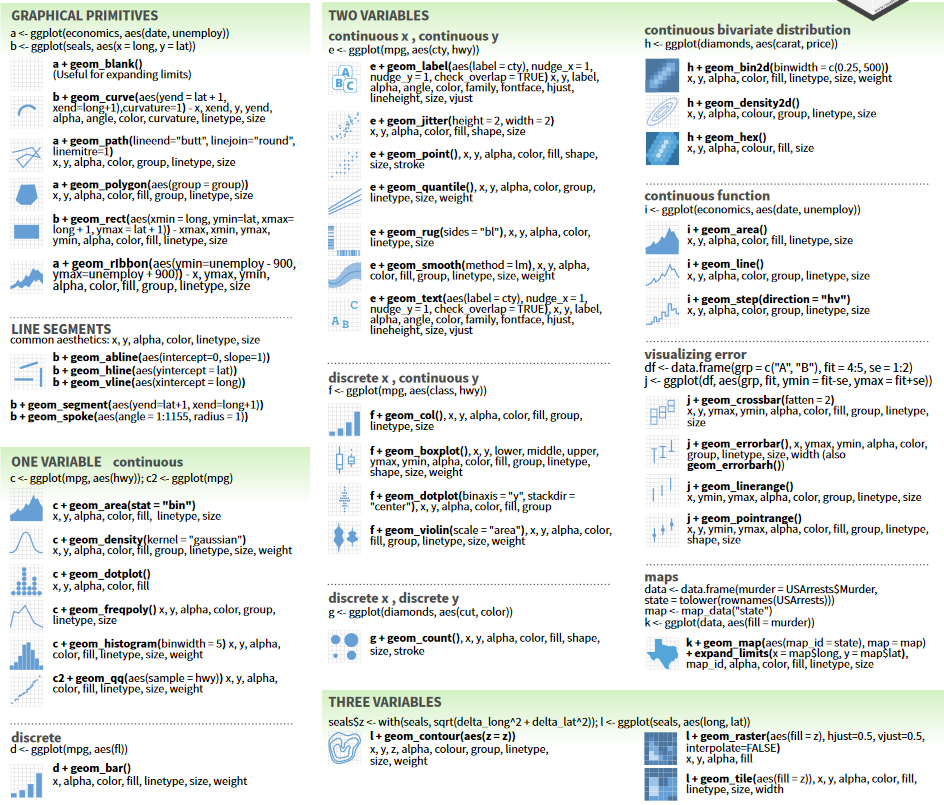
\includegraphics[width=13.11in,height=1\textheight]{images/geoms} \end{center}
\end{frame}

\begin{frame}{Report - \texttt{rmarkdown}}
\protect\hypertarget{report---rmarkdown}{}
\begin{itemize}
\tightlist
\item
  Easily interweave code, \(\LaTeX\) and text.
\item
  Render as reports (.html, .docx, .pdf), slides (.html, .ppt), or web
  applications (Shiny)
\item
  Example: these slides
\item
  Your PI will love you
\item
  Demonstration at end of session 1 if there's time
\end{itemize}


\includegraphics[width=0.9\linewidth]{images/rmd}
\end{frame}

\begin{frame}{COVID data}
\protect\hypertarget{covid-data}{}
\begin{itemize}
\tightlist
\item
  New York Times COVID-19 data on Github
\item
  Provides COVID-19 data by county, state, and nation-wide
\item
  \url{https://github.com/nytimes/covid-19-data}
\end{itemize}
\end{frame}

\begin{frame}[fragile]{Example: US COVID-19 state-level data}
\protect\hypertarget{example-us-covid-19-state-level-data}{}
\begin{Shaded}
\begin{Highlighting}[]
\NormalTok{nyt\_url }\OtherTok{=} \StringTok{"https://raw.githubusercontent.com/nytimes/covid{-}19{-}data/master/us{-}states.csv"}
\NormalTok{state\_covid }\OtherTok{=} \FunctionTok{read\_csv}\NormalTok{(nyt\_url)}
\end{Highlighting}
\end{Shaded}

\begin{verbatim}
## 
## -- Column specification --------------------------------------------------------
## cols(
##   date = col_date(format = ""),
##   state = col_character(),
##   fips = col_character(),
##   cases = col_double(),
##   deaths = col_double()
## )
\end{verbatim}
\end{frame}

\begin{frame}[fragile]{Example: US COVID-19 state-level data}
\protect\hypertarget{example-us-covid-19-state-level-data-1}{}
\begin{Shaded}
\begin{Highlighting}[]
\NormalTok{state\_covid}
\end{Highlighting}
\end{Shaded}

\begin{verbatim}
## # A tibble: 21,024 x 5
##    date       state      fips  cases deaths
##    <date>     <chr>      <chr> <dbl>  <dbl>
##  1 2020-01-21 Washington 53        1      0
##  2 2020-01-22 Washington 53        1      0
##  3 2020-01-23 Washington 53        1      0
##  4 2020-01-24 Illinois   17        1      0
##  5 2020-01-24 Washington 53        1      0
##  6 2020-01-25 California 06        1      0
##  7 2020-01-25 Illinois   17        1      0
##  8 2020-01-25 Washington 53        1      0
##  9 2020-01-26 Arizona    04        1      0
## 10 2020-01-26 California 06        2      0
## # ... with 21,014 more rows
\end{verbatim}
\end{frame}

\begin{frame}[fragile]{Example: US COVID-19}
\protect\hypertarget{example-us-covid-19}{}
\begin{Shaded}
\begin{Highlighting}[]
\NormalTok{state\_covid }\SpecialCharTok{\%\textgreater{}\%} 
  \FunctionTok{filter}\NormalTok{(state }\SpecialCharTok{==} \StringTok{"Washington"}\NormalTok{) }\SpecialCharTok{\%\textgreater{}\%} 
  \FunctionTok{mutate}\NormalTok{(}\AttributeTok{new\_deaths =} \FunctionTok{c}\NormalTok{(}\ConstantTok{NA}\NormalTok{, }\FunctionTok{diff}\NormalTok{(deaths))) }\SpecialCharTok{\%\textgreater{}\%} 
  \FunctionTok{ggplot}\NormalTok{(}\FunctionTok{aes}\NormalTok{(date, new\_deaths)) }\SpecialCharTok{+}
  \FunctionTok{geom\_point}\NormalTok{() }\SpecialCharTok{+} 
  \FunctionTok{geom\_smooth}\NormalTok{(}\AttributeTok{method =} \StringTok{"loess"}\NormalTok{, }\AttributeTok{span =}\NormalTok{ .}\DecValTok{2}\NormalTok{) }\SpecialCharTok{+} 
  \FunctionTok{labs}\NormalTok{(}\AttributeTok{title =} \StringTok{"Daily new deaths in Washington"}\NormalTok{,}
       \AttributeTok{y =} \StringTok{"New Deaths"}\NormalTok{,}
       \AttributeTok{caption =} \StringTok{"Data from the New York Times: https://github.com/nytimes/covid{-}19{-}data"}\NormalTok{) }\SpecialCharTok{+} 
  \FunctionTok{theme\_bw}\NormalTok{()}
\end{Highlighting}
\end{Shaded}

\begin{itemize}
\tightlist
\item
  What will the output of this command look like?
\end{itemize}
\end{frame}

\begin{frame}{Example: US COVID-19}
\protect\hypertarget{example-us-covid-19-1}{}
\includegraphics[width=0.9\linewidth]{tidy_overview_files/figure-beamer/unnamed-chunk-36-1}
\end{frame}

\hypertarget{day-2}{%
\section{Day 2}\label{day-2}}

\begin{frame}{\texttt{purrr}}
\protect\hypertarget{purrr}{}
\begin{itemize}
\tightlist
\item
  Functional programming
\end{itemize}
\end{frame}

\begin{frame}[fragile]{\texttt{map()}}
\protect\hypertarget{map}{}
\begin{itemize}
\tightlist
\item
  Apply a function to each element of a list
\item
  Example:
\end{itemize}

\begin{Shaded}
\begin{Highlighting}[]
\FunctionTok{map}\NormalTok{(}\DecValTok{1}\SpecialCharTok{:}\DecValTok{3}\NormalTok{, sqrt)}
\end{Highlighting}
\end{Shaded}

\begin{verbatim}
## [[1]]
## [1] 1
## 
## [[2]]
## [1] 1.414214
## 
## [[3]]
## [1] 1.732051
\end{verbatim}
\end{frame}

\begin{frame}[fragile]{\texttt{map()}}
\protect\hypertarget{map-1}{}
\begin{itemize}
\tightlist
\item
  Apply a function to each element of a list
\item
  Example:
\end{itemize}

\begin{Shaded}
\begin{Highlighting}[]
\FunctionTok{map}\NormalTok{(}\DecValTok{1}\SpecialCharTok{:}\DecValTok{3}\NormalTok{, sqrt)}
\end{Highlighting}
\end{Shaded}

\begin{verbatim}
## [[1]]
## [1] 1
## 
## [[2]]
## [1] 1.414214
## 
## [[3]]
## [1] 1.732051
\end{verbatim}

\begin{Shaded}
\begin{Highlighting}[]
\FunctionTok{map}\NormalTok{(datasets, ml\_algorithm)}
\end{Highlighting}
\end{Shaded}
\end{frame}

\begin{frame}[fragile]{Anonymous functions}
\protect\hypertarget{anonymous-functions}{}
\begin{itemize}
\tightlist
\item
  Tilde + \texttt{.x}
\item
  Use to easily define single-use functions
\end{itemize}
\end{frame}

\begin{frame}[fragile]{\texttt{map\_*()} variants}
\protect\hypertarget{map_-variants}{}
\begin{itemize}
\tightlist
\item
  \texttt{map()} always returns a list
\item
  Variants return a vector of a specific type
\end{itemize}

\begin{Shaded}
\begin{Highlighting}[]
\FunctionTok{map\_dbl}\NormalTok{(}\DecValTok{1}\SpecialCharTok{:}\DecValTok{5}\NormalTok{, }\SpecialCharTok{\textasciitilde{}}\NormalTok{.x}\SpecialCharTok{\^{}}\DecValTok{2} \SpecialCharTok{+} \DecValTok{1}\NormalTok{)}
\end{Highlighting}
\end{Shaded}

\begin{verbatim}
## [1]  2  5 10 17 26
\end{verbatim}

\begin{Shaded}
\begin{Highlighting}[]
\FunctionTok{map\_lgl}\NormalTok{(}\DecValTok{1}\SpecialCharTok{:}\DecValTok{5}\NormalTok{, }\SpecialCharTok{\textasciitilde{}}\NormalTok{.x }\SpecialCharTok{==} \DecValTok{3}\NormalTok{)}
\end{Highlighting}
\end{Shaded}

\begin{verbatim}
## [1] FALSE FALSE  TRUE FALSE FALSE
\end{verbatim}

\begin{Shaded}
\begin{Highlighting}[]
\FunctionTok{map\_chr}\NormalTok{(letters[}\DecValTok{1}\SpecialCharTok{:}\DecValTok{5}\NormalTok{], }\SpecialCharTok{\textasciitilde{}}\FunctionTok{paste0}\NormalTok{(}\FunctionTok{rep}\NormalTok{(.x, }\DecValTok{3}\NormalTok{), }\AttributeTok{collapse=}\StringTok{\textquotesingle{}\textquotesingle{}}\NormalTok{))}
\end{Highlighting}
\end{Shaded}

\begin{verbatim}
## [1] "aaa" "bbb" "ccc" "ddd" "eee"
\end{verbatim}
\end{frame}

\begin{frame}[fragile]{purrr example: run many models}
\protect\hypertarget{purrr-example-run-many-models}{}
\begin{itemize}
\tightlist
\item
  Define each combination of two explanatory variables
\end{itemize}

\begin{Shaded}
\begin{Highlighting}[]
\NormalTok{formula\_df }\OtherTok{=} \FunctionTok{names}\NormalTok{(diabetes)[}\DecValTok{1}\SpecialCharTok{:}\DecValTok{7}\NormalTok{] }\SpecialCharTok{\%\textgreater{}\%} 
  \FunctionTok{combn}\NormalTok{(}\AttributeTok{m =} \DecValTok{2}\NormalTok{) }\SpecialCharTok{\%\textgreater{}\%} 
\NormalTok{  t }\SpecialCharTok{\%\textgreater{}\%} 
\NormalTok{  as\_tibble }\SpecialCharTok{\%\textgreater{}\%} 
  \FunctionTok{set\_names}\NormalTok{(}\FunctionTok{c}\NormalTok{(}\StringTok{\textquotesingle{}x1\textquotesingle{}}\NormalTok{, }\StringTok{\textquotesingle{}x2\textquotesingle{}}\NormalTok{)) }\SpecialCharTok{\%\textgreater{}\%} 
  \FunctionTok{mutate}\NormalTok{(}\AttributeTok{formula =} \FunctionTok{paste}\NormalTok{(}\StringTok{"diabetic \textasciitilde{} "}\NormalTok{, x1, }\StringTok{" + "}\NormalTok{, x2, }\AttributeTok{sep =} \StringTok{\textquotesingle{}\textquotesingle{}}\NormalTok{))}
\end{Highlighting}
\end{Shaded}

\begin{verbatim}
## Warning: The `x` argument of `as_tibble.matrix()` must have unique column names if `.name_repair` is omitted as of tibble 2.0.0.
## Using compatibility `.name_repair`.
## This warning is displayed once every 8 hours.
## Call `lifecycle::last_warnings()` to see where this warning was generated.
\end{verbatim}

\begin{Shaded}
\begin{Highlighting}[]
\NormalTok{formula\_df}
\end{Highlighting}
\end{Shaded}

\begin{verbatim}
## # A tibble: 21 x 3
##    x1    x2    formula                
##    <chr> <chr> <chr>                  
##  1 npreg glu   diabetic ~ npreg + glu 
##  2 npreg bp    diabetic ~ npreg + bp  
##  3 npreg skin  diabetic ~ npreg + skin
##  4 npreg bmi   diabetic ~ npreg + bmi 
##  5 npreg ped   diabetic ~ npreg + ped 
##  6 npreg age   diabetic ~ npreg + age 
##  7 glu   bp    diabetic ~ glu + bp    
##  8 glu   skin  diabetic ~ glu + skin  
##  9 glu   bmi   diabetic ~ glu + bmi   
## 10 glu   ped   diabetic ~ glu + ped   
## # ... with 11 more rows
\end{verbatim}
\end{frame}

\begin{frame}[fragile]{purrr example: run many models}
\protect\hypertarget{purrr-example-run-many-models-1}{}
\begin{itemize}
\tightlist
\item
  Run a logistic regression on each combination of explanatory variables
\end{itemize}

\begin{Shaded}
\begin{Highlighting}[]
\NormalTok{formula\_df }\SpecialCharTok{\%\textgreater{}\%} 
  \FunctionTok{mutate}\NormalTok{(}\AttributeTok{glm\_result =} \FunctionTok{map}\NormalTok{(formula,}
                          \SpecialCharTok{\textasciitilde{}}\FunctionTok{glm}\NormalTok{(.x, }\AttributeTok{data =}\NormalTok{ diabetes, }\AttributeTok{family =} \StringTok{\textquotesingle{}binomial\textquotesingle{}}\NormalTok{))) }
\end{Highlighting}
\end{Shaded}
\end{frame}

\begin{frame}[fragile]{purrr example: run many models}
\protect\hypertarget{purrr-example-run-many-models-2}{}
\begin{itemize}
\tightlist
\item
  Extract the AIC of each model fit
\end{itemize}

\begin{Shaded}
\begin{Highlighting}[]
\NormalTok{formula\_df }\SpecialCharTok{\%\textgreater{}\%} 
  \FunctionTok{mutate}\NormalTok{(}\AttributeTok{glm\_result =} \FunctionTok{map}\NormalTok{(formula,}
                          \SpecialCharTok{\textasciitilde{}}\FunctionTok{glm}\NormalTok{(.x, }\AttributeTok{data =}\NormalTok{ diabetes, }\AttributeTok{family =} \StringTok{\textquotesingle{}binomial\textquotesingle{}}\NormalTok{)),}
         \AttributeTok{aic =} \FunctionTok{map\_dbl}\NormalTok{(lm\_result,}
                       \SpecialCharTok{\textasciitilde{}}\NormalTok{.x}\SpecialCharTok{$}\NormalTok{aic)) }
\end{Highlighting}
\end{Shaded}
\end{frame}

\begin{frame}[fragile]{purrr example: run many models}
\protect\hypertarget{purrr-example-run-many-models-3}{}
\begin{itemize}
\tightlist
\item
  See which model had the lowest AIC
\end{itemize}

\begin{Shaded}
\begin{Highlighting}[]
\NormalTok{formula\_df }\SpecialCharTok{\%\textgreater{}\%} 
  \FunctionTok{mutate}\NormalTok{(}\AttributeTok{glm\_result =} \FunctionTok{map}\NormalTok{(formula,}
                          \SpecialCharTok{\textasciitilde{}}\FunctionTok{glm}\NormalTok{(.x, }\AttributeTok{data =}\NormalTok{ diabetes, }\AttributeTok{family =} \StringTok{\textquotesingle{}binomial\textquotesingle{}}\NormalTok{)),}
         \AttributeTok{aic =} \FunctionTok{map\_dbl}\NormalTok{(lm\_result,}
                       \SpecialCharTok{\textasciitilde{}}\NormalTok{.x}\SpecialCharTok{$}\NormalTok{aic)) }\SpecialCharTok{\%\textgreater{}\%} 
  \FunctionTok{arrange}\NormalTok{(aic)}
\end{Highlighting}
\end{Shaded}
\end{frame}

\begin{frame}[fragile]{Organize - \texttt{tidyr}}
\protect\hypertarget{organize---tidyr}{}
\begin{itemize}
\tightlist
\item
  \texttt{pivot\_longer()} and \texttt{pivot\_wider()}
\item
  \texttt{separate()} and \texttt{unite()}
\end{itemize}
\end{frame}

\begin{frame}[fragile]{Data tidying example: WHO TB data}
\protect\hypertarget{data-tidying-example-who-tb-data}{}
\begin{itemize}
\tightlist
\item
  WHO tuberculosis case data
\item
  realistically messy!
\item
  Try running these commands:
\end{itemize}

\begin{Shaded}
\begin{Highlighting}[]
\NormalTok{?tidyr}\SpecialCharTok{::}\NormalTok{who}
\FunctionTok{dim}\NormalTok{(who)}
\FunctionTok{names}\NormalTok{(who)}
\NormalTok{who[}\DecValTok{1}\SpecialCharTok{:}\DecValTok{5}\NormalTok{, }\DecValTok{1}\SpecialCharTok{:}\DecValTok{8}\NormalTok{]}
\NormalTok{who}
\end{Highlighting}
\end{Shaded}

\begin{itemize}
\tightlist
\item
  We will tidy this data in 5 steps
\end{itemize}
\end{frame}

\begin{frame}{WHO TB column names}
\protect\hypertarget{who-tb-column-names}{}
\begin{itemize}
\tightlist
\item
  First part: ``new'' or ``old''
\item
  Second part: TB type (relapse, extrapulmonary, smear-positive,
  smear-negative)
\item
  Third part: Sex and age group (e.g.~f2534)
\end{itemize}
\end{frame}

\begin{frame}[fragile]{TB tidying 1/5: pivot wide to long}
\protect\hypertarget{tb-tidying-15-pivot-wide-to-long}{}
\begin{Shaded}
\begin{Highlighting}[]
\NormalTok{who1 }\OtherTok{=}\NormalTok{ who }\SpecialCharTok{\%\textgreater{}\%} 
  \FunctionTok{pivot\_longer}\NormalTok{(new\_sp\_m014}\SpecialCharTok{:}\NormalTok{newrel\_f65, }
               \AttributeTok{names\_to =} \StringTok{"key"}\NormalTok{, }
               \AttributeTok{values\_to =} \StringTok{"values"}\NormalTok{, }
               \AttributeTok{values\_drop\_na =} \ConstantTok{TRUE}\NormalTok{)}
\NormalTok{who1}
\end{Highlighting}
\end{Shaded}

\begin{verbatim}
## # A tibble: 76,046 x 6
##    country     iso2  iso3   year key          values
##    <chr>       <chr> <chr> <int> <chr>         <int>
##  1 Afghanistan AF    AFG    1997 new_sp_m014       0
##  2 Afghanistan AF    AFG    1997 new_sp_m1524     10
##  3 Afghanistan AF    AFG    1997 new_sp_m2534      6
##  4 Afghanistan AF    AFG    1997 new_sp_m3544      3
##  5 Afghanistan AF    AFG    1997 new_sp_m4554      5
##  6 Afghanistan AF    AFG    1997 new_sp_m5564      2
##  7 Afghanistan AF    AFG    1997 new_sp_m65        0
##  8 Afghanistan AF    AFG    1997 new_sp_f014       5
##  9 Afghanistan AF    AFG    1997 new_sp_f1524     38
## 10 Afghanistan AF    AFG    1997 new_sp_f2534     36
## # ... with 76,036 more rows
\end{verbatim}
\end{frame}

\begin{frame}[fragile]{TB tidying 2/5: fix inconsistent names}
\protect\hypertarget{tb-tidying-25-fix-inconsistent-names}{}
\begin{Shaded}
\begin{Highlighting}[]
\NormalTok{who2 }\OtherTok{=}\NormalTok{ who1 }\SpecialCharTok{\%\textgreater{}\%} 
  \FunctionTok{mutate}\NormalTok{(}\AttributeTok{key =} \FunctionTok{str\_replace}\NormalTok{(key, }\StringTok{"newrel"}\NormalTok{, }\StringTok{"new\_rel"}\NormalTok{))}
\NormalTok{who2}
\end{Highlighting}
\end{Shaded}

\begin{verbatim}
## # A tibble: 76,046 x 6
##    country     iso2  iso3   year key          values
##    <chr>       <chr> <chr> <int> <chr>         <int>
##  1 Afghanistan AF    AFG    1997 new_sp_m014       0
##  2 Afghanistan AF    AFG    1997 new_sp_m1524     10
##  3 Afghanistan AF    AFG    1997 new_sp_m2534      6
##  4 Afghanistan AF    AFG    1997 new_sp_m3544      3
##  5 Afghanistan AF    AFG    1997 new_sp_m4554      5
##  6 Afghanistan AF    AFG    1997 new_sp_m5564      2
##  7 Afghanistan AF    AFG    1997 new_sp_m65        0
##  8 Afghanistan AF    AFG    1997 new_sp_f014       5
##  9 Afghanistan AF    AFG    1997 new_sp_f1524     38
## 10 Afghanistan AF    AFG    1997 new_sp_f2534     36
## # ... with 76,036 more rows
\end{verbatim}
\end{frame}

\begin{frame}[fragile]{TB tidying 3/5: separate identifier components}
\protect\hypertarget{tb-tidying-35-separate-identifier-components}{}
\begin{Shaded}
\begin{Highlighting}[]
\NormalTok{who3 }\OtherTok{=}\NormalTok{ who2 }\SpecialCharTok{\%\textgreater{}\%} 
  \FunctionTok{separate}\NormalTok{(key, }\AttributeTok{into =} \FunctionTok{c}\NormalTok{(}\StringTok{"newold"}\NormalTok{, }\StringTok{"tb\_type"}\NormalTok{, }\StringTok{"sexage"}\NormalTok{))}
\end{Highlighting}
\end{Shaded}
\end{frame}

\begin{frame}[fragile]{TB tidying 4/5: separate sex and age group}
\protect\hypertarget{tb-tidying-45-separate-sex-and-age-group}{}
\begin{Shaded}
\begin{Highlighting}[]
\NormalTok{who4 }\OtherTok{=}\NormalTok{ who3 }\SpecialCharTok{\%\textgreater{}\%} 
  \FunctionTok{separate}\NormalTok{(sexage, }\AttributeTok{into =} \FunctionTok{c}\NormalTok{(}\StringTok{"sex"}\NormalTok{, }\StringTok{"age\_group"}\NormalTok{), }\AttributeTok{sep =} \DecValTok{1}\NormalTok{)}
\end{Highlighting}
\end{Shaded}
\end{frame}

\begin{frame}[fragile]{TB tidying 5/5: remove redundant columns}
\protect\hypertarget{tb-tidying-55-remove-redundant-columns}{}
\begin{Shaded}
\begin{Highlighting}[]
\NormalTok{who\_final }\OtherTok{=}\NormalTok{ who4 }\SpecialCharTok{\%\textgreater{}\%} 
  \FunctionTok{select}\NormalTok{(}\SpecialCharTok{{-}}\NormalTok{newold, }\SpecialCharTok{{-}}\FunctionTok{matches}\NormalTok{(}\StringTok{"iso"}\NormalTok{))}
\end{Highlighting}
\end{Shaded}
\end{frame}

\begin{frame}[fragile]{TB tidying: Final command}
\protect\hypertarget{tb-tidying-final-command}{}
\begin{Shaded}
\begin{Highlighting}[]
\NormalTok{tidyr}\SpecialCharTok{::}\NormalTok{who }\SpecialCharTok{\%\textgreater{}\%} 
  \FunctionTok{pivot\_longer}\NormalTok{(new\_sp\_m014}\SpecialCharTok{:}\NormalTok{newrel\_f65, }
               \AttributeTok{names\_to =} \StringTok{"key"}\NormalTok{, }
               \AttributeTok{values\_to =} \StringTok{"values"}\NormalTok{, }
               \AttributeTok{values\_drop\_na =} \ConstantTok{TRUE}\NormalTok{) }\SpecialCharTok{\%\textgreater{}\%}
  \FunctionTok{mutate}\NormalTok{(}\AttributeTok{key =} \FunctionTok{str\_replace}\NormalTok{(key, }\StringTok{"newrel"}\NormalTok{, }\StringTok{"new\_rel"}\NormalTok{)) }\SpecialCharTok{\%\textgreater{}\%}
  \FunctionTok{separate}\NormalTok{(key, }\AttributeTok{into =} \FunctionTok{c}\NormalTok{(}\StringTok{"newold"}\NormalTok{, }\StringTok{"tb\_type"}\NormalTok{, }\StringTok{"sexage"}\NormalTok{)) }\SpecialCharTok{\%\textgreater{}\%} 
  \FunctionTok{separate}\NormalTok{(sexage, }\AttributeTok{into =} \FunctionTok{c}\NormalTok{(}\StringTok{"sex"}\NormalTok{, }\StringTok{"age\_group"}\NormalTok{), }\AttributeTok{sep =} \DecValTok{1}\NormalTok{) }\SpecialCharTok{\%\textgreater{}\%} 
  \FunctionTok{select}\NormalTok{(}\SpecialCharTok{{-}}\NormalTok{newold, }\SpecialCharTok{{-}}\FunctionTok{matches}\NormalTok{(}\StringTok{"iso"}\NormalTok{))}
\end{Highlighting}
\end{Shaded}

\begin{verbatim}
## # A tibble: 76,046 x 6
##    country      year tb_type sex   age_group values
##    <chr>       <int> <chr>   <chr> <chr>      <int>
##  1 Afghanistan  1997 sp      m     014            0
##  2 Afghanistan  1997 sp      m     1524          10
##  3 Afghanistan  1997 sp      m     2534           6
##  4 Afghanistan  1997 sp      m     3544           3
##  5 Afghanistan  1997 sp      m     4554           5
##  6 Afghanistan  1997 sp      m     5564           2
##  7 Afghanistan  1997 sp      m     65             0
##  8 Afghanistan  1997 sp      f     014            5
##  9 Afghanistan  1997 sp      f     1524          38
## 10 Afghanistan  1997 sp      f     2534          36
## # ... with 76,036 more rows
\end{verbatim}
\end{frame}

\begin{frame}{Joins if there's time}
\protect\hypertarget{joins-if-theres-time}{}
\end{frame}

\begin{frame}[fragile]{Everything else}
\protect\hypertarget{everything-else}{}
\begin{itemize}
\tightlist
\item
  \texttt{forcats}
\item
  \texttt{stringr}
\item
  \texttt{lubridate}
\item
  \texttt{tidymodels}
\end{itemize}
\end{frame}

\begin{frame}{Resources}
\protect\hypertarget{resources}{}
\begin{itemize}
\tightlist
\item
  \href{https://r4ds.had.co.nz/}{R for Data Science -
  https://r4ds.had.co.nz/}
\item
  \href{https://rstudio.com/resources/cheatsheets/}{Cheat Sheets -
  https://rstudio.com/resources/cheatsheets/}
\end{itemize}
\end{frame}

\end{document}
